\begin{figure}[!htbp]
\caption{Legislator Ideal Points and District Ideology Means}
\begin{centering}
%\centering
%\fbox{
  \begin{tabular}{@{}ccc@{}}
	% & & \\  	
  	\small (A) Ideal Point &
    \small (B) Ideal Point &
    \small (C) Ideal Point  \\
    \small vs District Ideology & 
    \small vs Same-Party Ideology &
    \small vs Non-Same-Party Ideology \\
    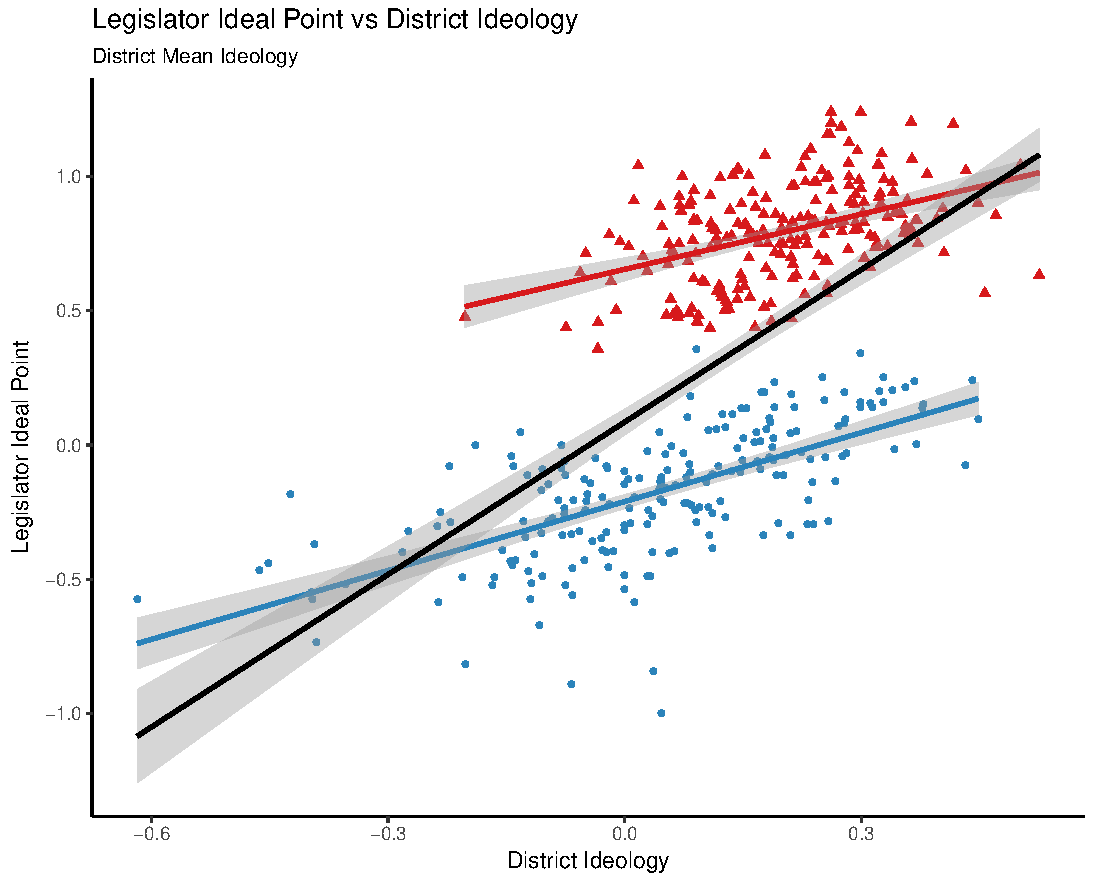
\includegraphics[width=.30\textwidth]{/Users/dsimp/GitHub/Clinton(2006)Rep/drafts/plots/plot1-1.pdf} &
    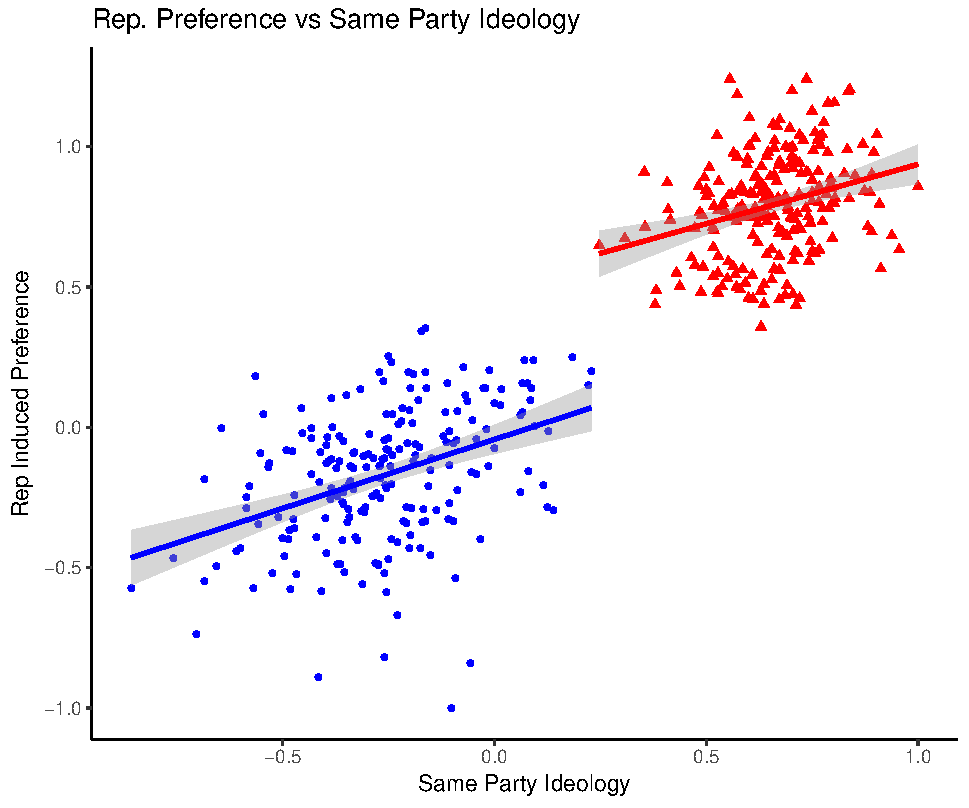
\includegraphics[width=.30\textwidth]{/Users/dsimp/GitHub/Clinton(2006)Rep/drafts/plots/plot1-2.pdf} &
    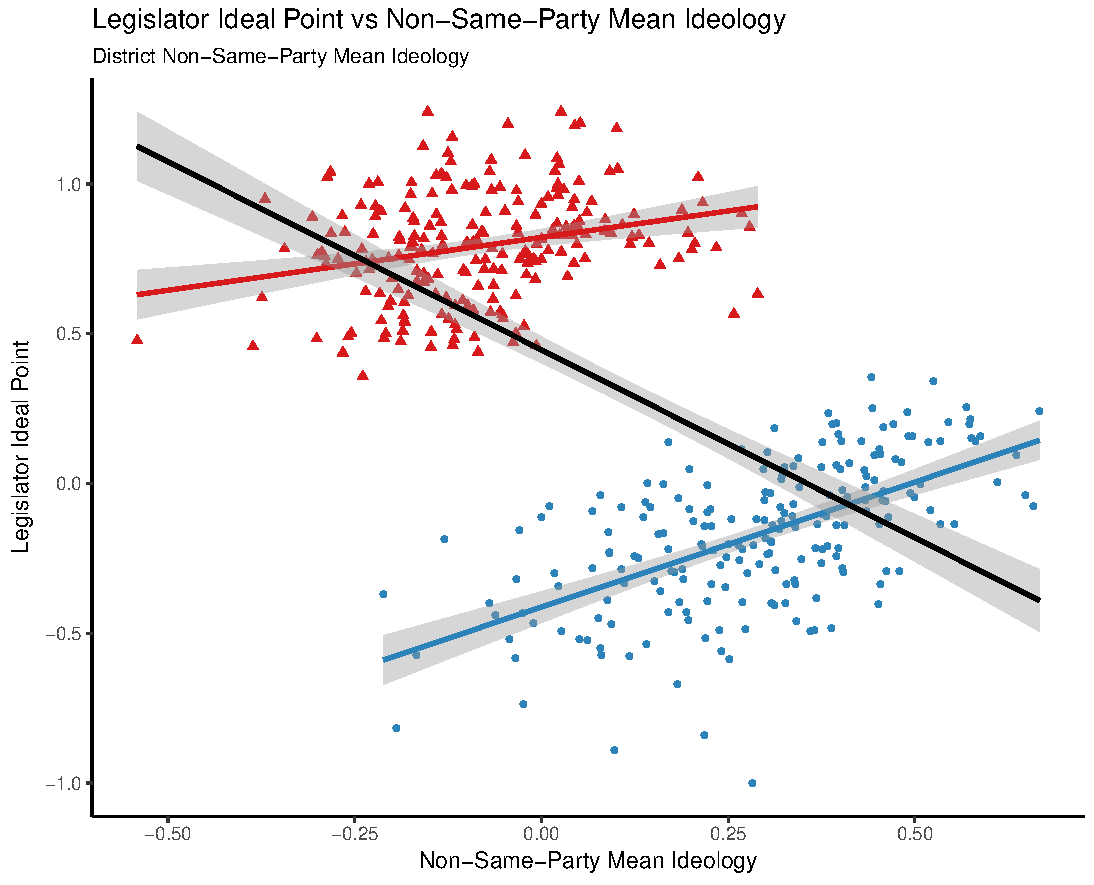
\includegraphics[width=.30\textwidth]{/Users/dsimp/GitHub/Clinton(2006)Rep/drafts/plots/plot1-3.pdf} \\
    % & & \\
    \small (D) Ideal Point & 
    \small (E) Ideal Point & 
    \small (F) Same-Party Ideology  \\
    \small vs Opposite Party Ideology  & 
    \small vs Independent Ideology  & 
    \small vs District Ideology \\
    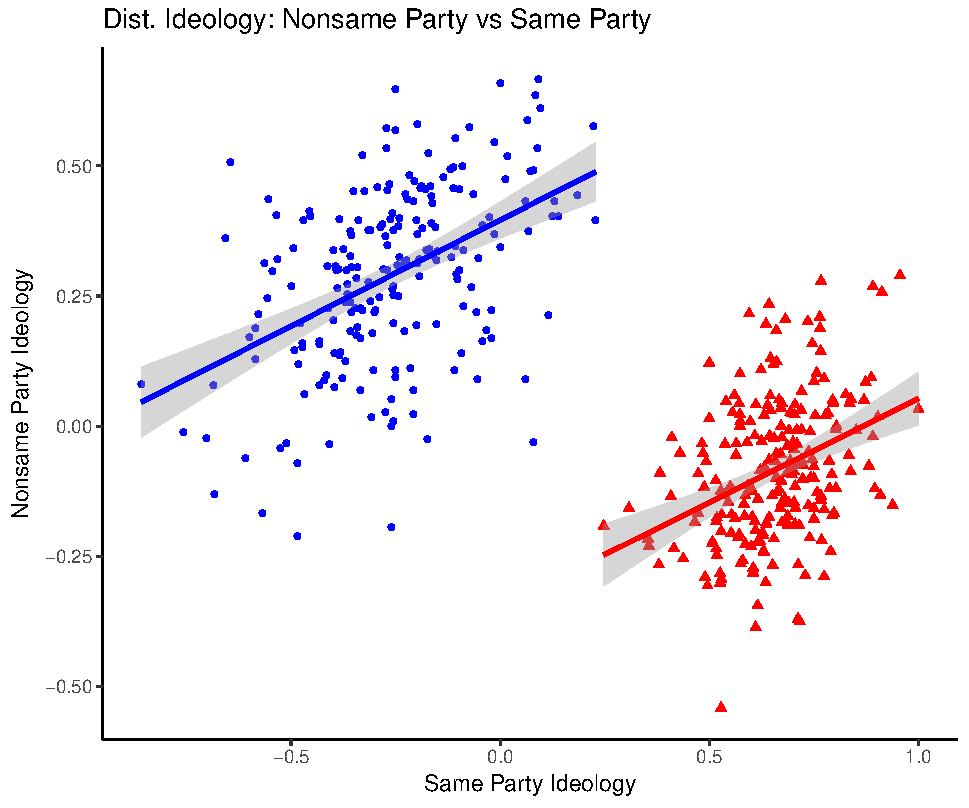
\includegraphics[width=.30\textwidth]{/Users/dsimp/GitHub/Clinton(2006)Rep/drafts/plots/plot1-4.pdf} &
    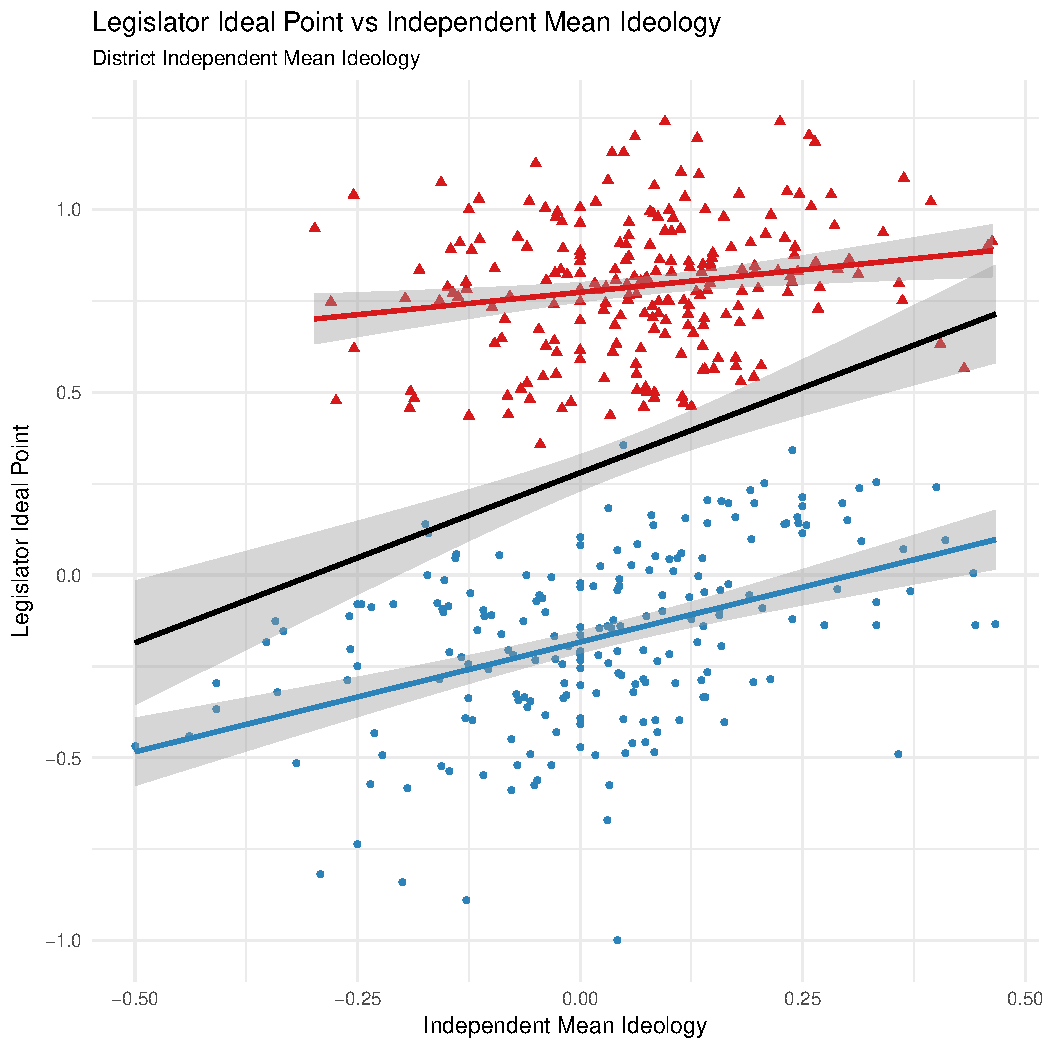
\includegraphics[width=.30\textwidth]{/Users/dsimp/GitHub/Clinton(2006)Rep/drafts/plots/plot1-5.pdf} &
    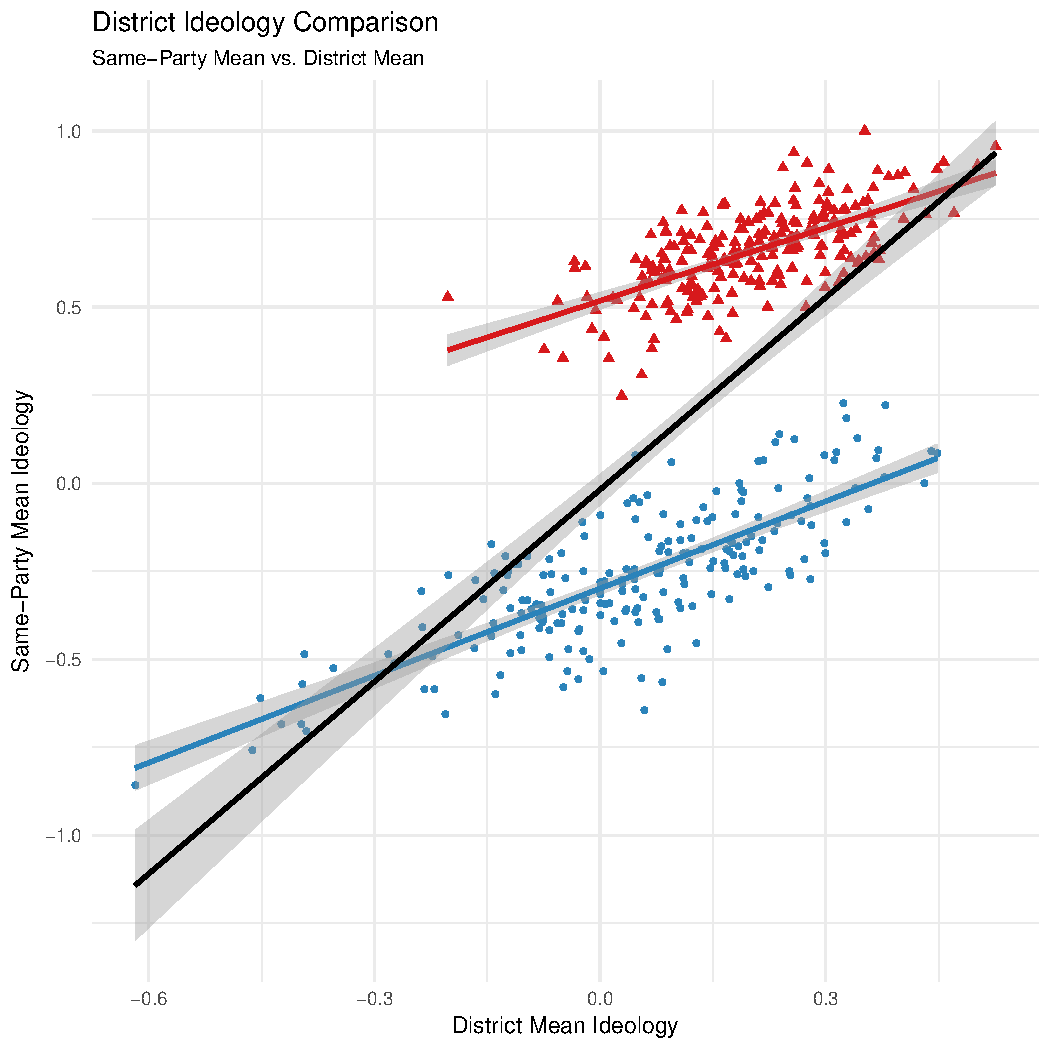
\includegraphics[width=.30\textwidth]{/Users/dsimp/GitHub/Clinton(2006)Rep/drafts/plots/plot1-6.pdf} \\
    % &  &\\
    \small (G) Non-Same-Party Ideology & 
    \small (H) Opposite Party Ideology & 
    \small (I) Independent Ideology  \\
    \small vs District Ideology  & 
    \small vs District Ideology  & 
    \small vs District Ideology \\
    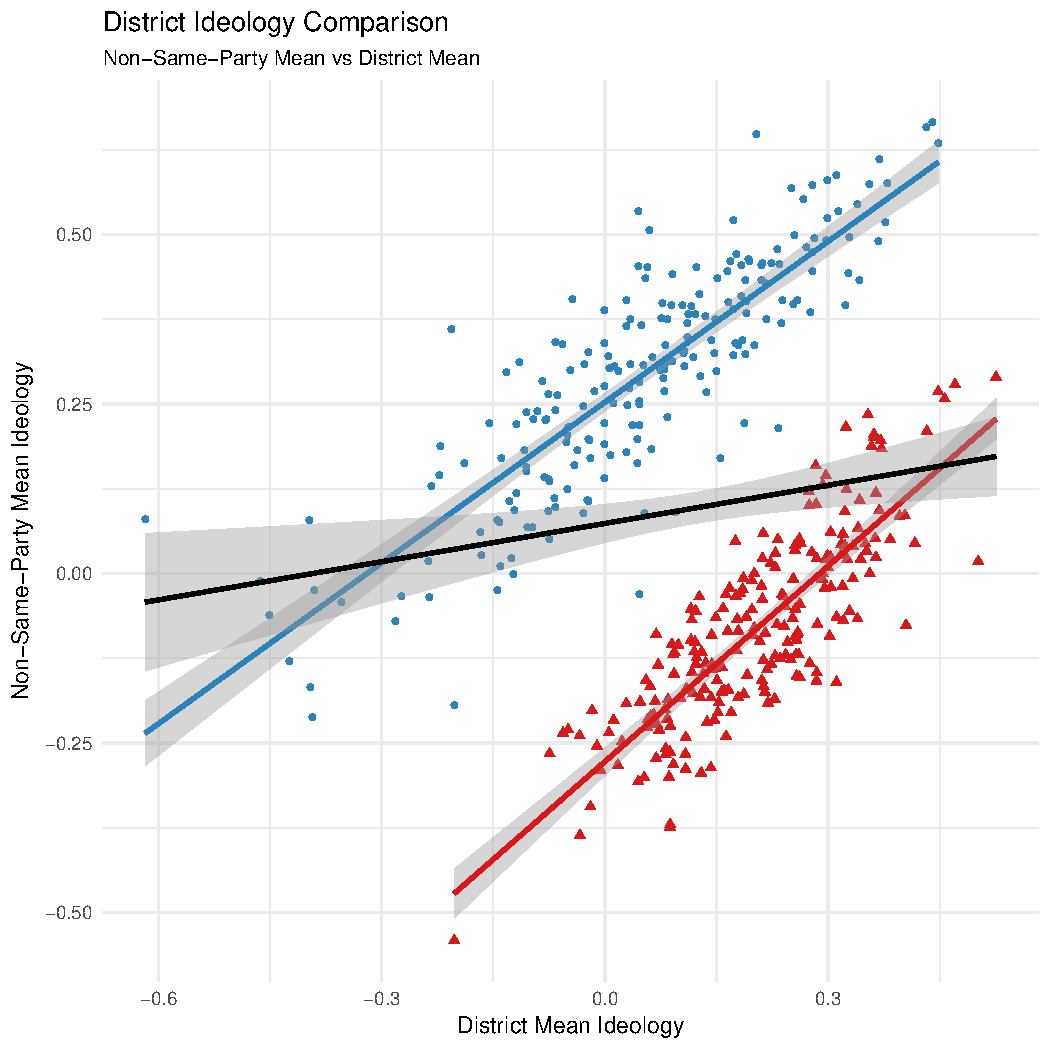
\includegraphics[width=.30\textwidth]{/Users/dsimp/GitHub/Clinton(2006)Rep/drafts/plots/plot1-7.pdf} &
    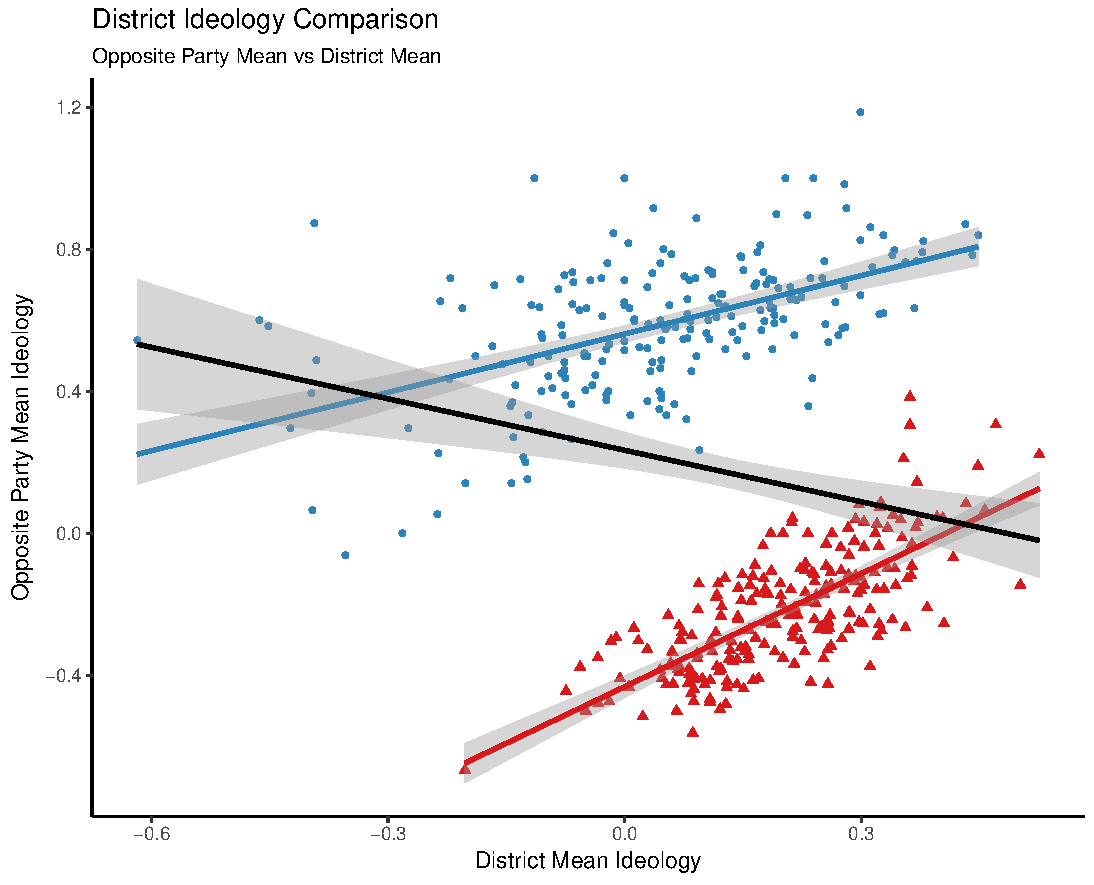
\includegraphics[width=.30\textwidth]{/Users/dsimp/GitHub/Clinton(2006)Rep/drafts/plots/plot1-8.pdf} &
    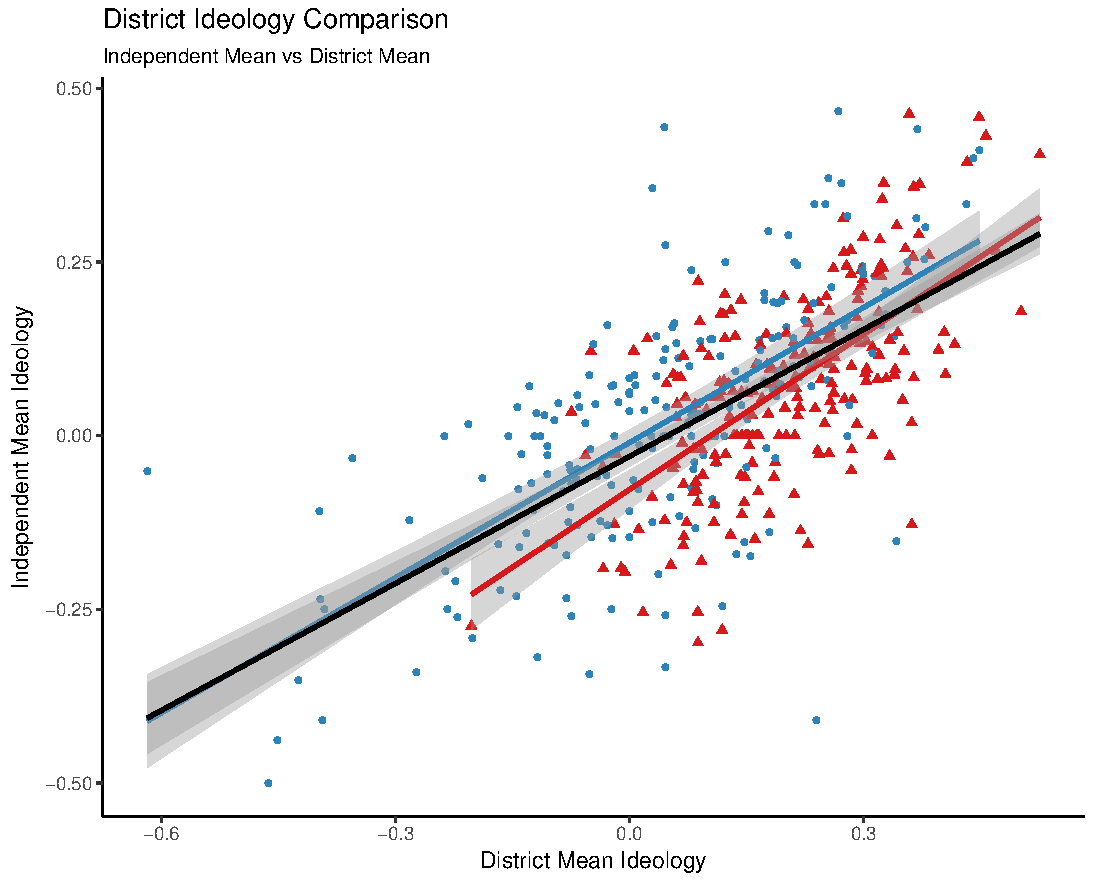
\includegraphics[width=.30\textwidth]{/Users/dsimp/GitHub/Clinton(2006)Rep/drafts/plots/plot1-9.pdf} \\
    % &  &\\
    \small (J) Non-Same-Party Ideology & 
    \small (K) Opposite Party Ideology & 
    \small (L) Independent Ideology  \\
    \small vs Same-Party Ideology  & 
    \small vs Same-Party Ideology  & 
    \small vs Same-Party Ideology \\
    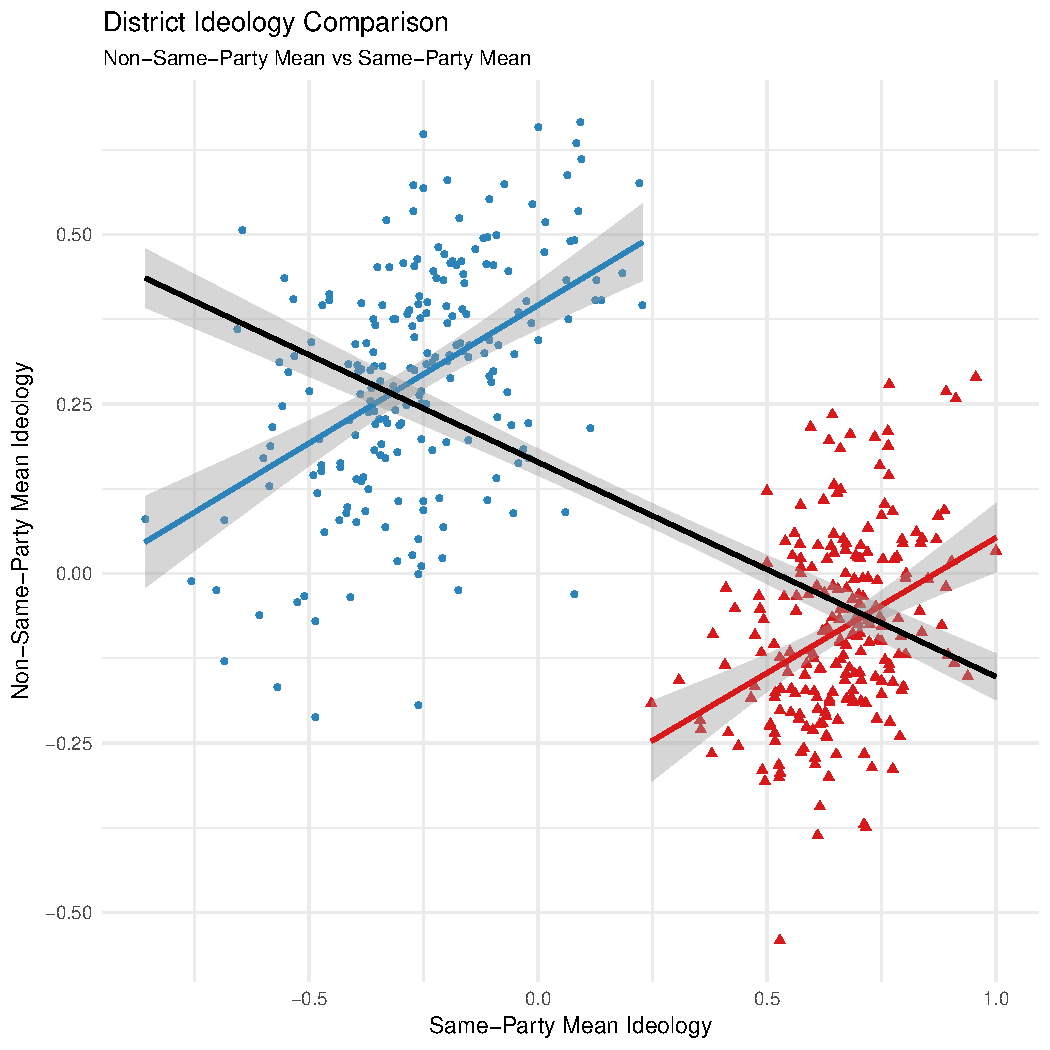
\includegraphics[width=.30\textwidth]{/Users/dsimp/GitHub/Clinton(2006)Rep/drafts/plots/plot1-10.pdf} &
    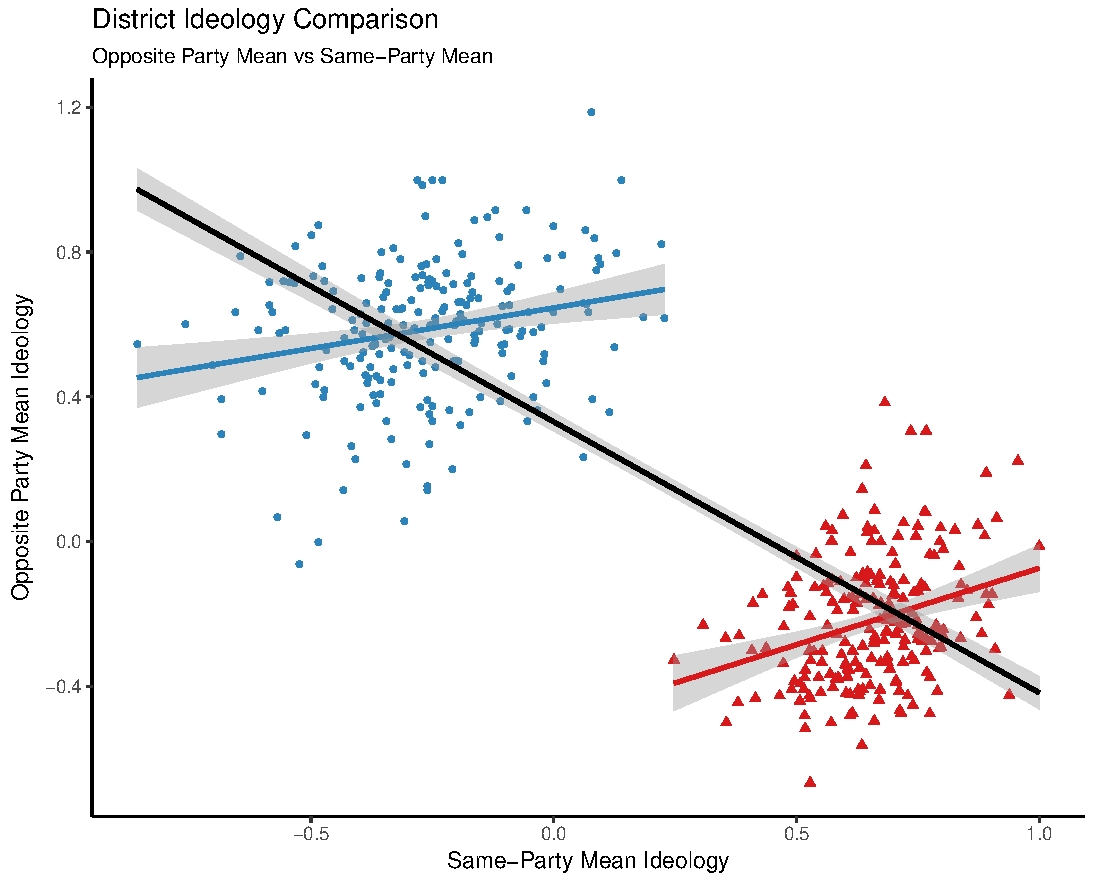
\includegraphics[width=.30\textwidth]{/Users/dsimp/GitHub/Clinton(2006)Rep/drafts/plots/plot1-11.pdf} &
    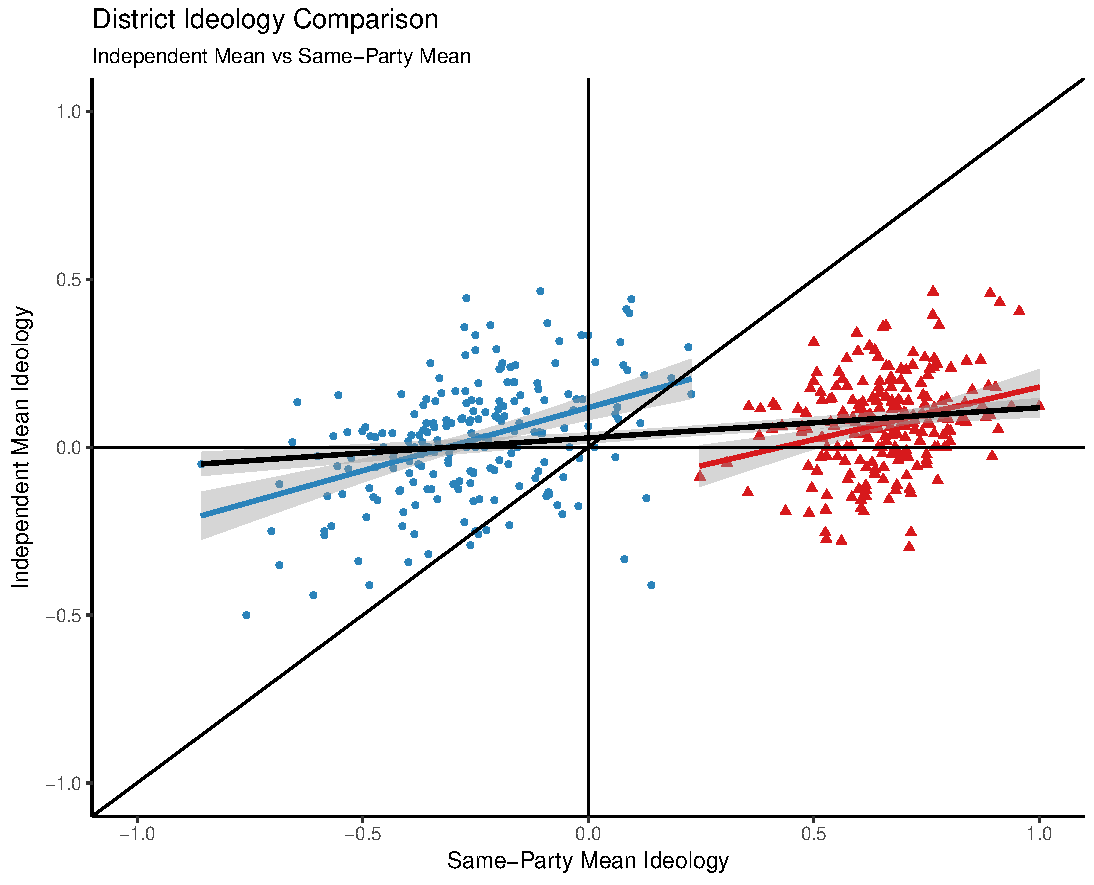
\includegraphics[width=.30\textwidth]{/Users/dsimp/GitHub/Clinton(2006)Rep/drafts/plots/plot1-12.pdf} \\
  \end{tabular}
    %}   
 \end{centering}
 \small \textbf{Note:} Districts represented by Republicans (Democrats) are plotted with triangles (circles). A bivariate trend line is plotted for overall comparison and party trend lines are plotted for comparison within districts.
\end{figure}